\documentclass[a4paper,10pt]{article}
\usepackage[dvips]{color,graphicx}
\usepackage[dvips, bookmarks, colorlinks=false]{hyperref}
\usepackage[all]{xy}

%opening
\title{Math508 Final Exam}
\author{Yu Huang}
\date{2007-05-07}

\begin{document}

\maketitle


\section{Problem 1}
For Ornstein-Uhlenbeck stationary sequence, $E X_n=0$, $R(k) = a^{|k|}$. The best linear estimate of $X_m$ given $X_k, X_{k-1}, X_{k-2}, ...$ is
\begin{equation}
\hat{X_m} = k_0 + k_1*X_k + k_2*X_{k-1} + k_3*X_{k-2} + ... \\
k_0 = EX_m = 0
\end{equation}

The matrices in the normal equation (\ref{normal_eq}) would be infinite although it could be easily be seen that $k_1=a^{m-k}$ while other $k$'s are all zero. Hence, $\hat{X_m} = a^{m-k}X_k$.

\begin{equation} \label{normal_eq}
\left( \begin{array}{cccc}
a^{0} & a^{1} & a^{2} & \ldots \\
a^{1} & a{0} & a^{1} & \ldots \\
\vdots & \vdots & \ddots
\end{array} \right)
\left(\begin{array}{c}
k_1 \\
k_2 \\
\vdots
\end{array} \right) = 
\left( \begin{array}{c}
a^{m-k} \\
a^{m-k+1} \\
\vdots
\end{array} \right)
\end{equation}


Instead guessing, i use the sequential project to prove this result. $M_n$ is a linear subspace generated by $\{1, X_k, X_{k-1}, \ldots, X{k-n+1}\}$.
\begin{equation}
\hat{X_{m,n}} = E(X_m|M_n)
\end{equation}
There's iteration that 
\begin{eqnarray}
\hat{X_{m,n}} = \hat{X_{m,n-1}} + \frac{c_{n,n-1}}{u_{n,n-1}}(X_{k-n}-X_{k-n+1}) \nonumber \\
\hat{X_{k-n,n-1}} = E(X_{k-n}|M_{n-1}) \nonumber \\
c_{n,n-1} = E[(X_m - \hat{X_{m,n-1}})(X_{k-n}-\hat{X_{k-n,n-1}})] \nonumber
\end{eqnarray}

Now take $n=2$, $M_2$ is a linear subspace generated by $\{1, X_k, X_{k-1}\}$ and $M_1$ is a linear subspace generated by $\{1, X_k\}$. We can get following results easily.
\begin{eqnarray}
\hat{X_{m,n-1}} = \hat{X_{m,1}} = a^{m-k}*X_k \\
\hat{X_{k-n,n-1}} = \hat{X_{k-1,1}} = aX_{k}
\end{eqnarray}

We can prove $c_{n,n-1}=0$.
\begin{eqnarray}
 c_{n,n-1} = c_{2,1} = E[(X_m - a^{m-k}*X_k)(X_{k-1} - aX_{k})] \nonumber \\
= E(X_m X_{k-1} - aX_mX_k - a^{m-k}X_kX_{k-1} + a^{m-k+1}X_kX_k) \nonumber\\
= a^{m-k+1} - a*a^{m-k} - a^{m-k}*a + a^{m-k+1} = 0 \\
\hat{X_{m,2}} = \hat{X_{m,1}} = a^{m-k}*X_k
\end{eqnarray}

By induction,
\begin{equation}
\hat{X_m} = a^{m-k}X_k
\end{equation}

\section{Problem 2}
\subsection{part a}
\begin{eqnarray}
P(X_{n+1} \leq u, Y_{n+1} \leq v | X_n=r, Y_n=s) \nonumber \\
= \int_{-\infty}^u P(Y_{n+1} \leq v | X_{n+1}=x) f(X_{n+1} = x|X_n=r, Y_n=s) dx \nonumber \\
= \int_{-\infty}^u \int_{-\infty}^v l(X_{n+1}=x, Y_{n+1}=y) p(X_{n+1}=x|X_n=r) dy dx \nonumber
\end{eqnarray}

Differentiate both sides by $\frac{\partial^2}{\partial u \partial v}$ to get the transition kernel
\begin{equation}
 q^{r,u}(s,v) = p(r,u)l(u,v)
\end{equation}

\subsection{part b}
Given $X_n=r$, if $W_n \geq -r$, $Y_n$ is distributed as $N(r,1)$. If $W_n < -r$, $Y_n$ is distributed as $N(-r,1)$. Graphically, $Y_n$'s distribution is a combination of $N(r,1)$ and $N(-r,1)$ with the only positive domain. So,
\begin{equation}
 P(Y_n<u|X_n=r) = \int_0^u \rho(y-r)dy + \int_0^u \rho(y+r)dy \nonumber
\end{equation}

$\rho(x)$ is the standard normal density function. Differentiate both sides by $\frac{\partial}{\partial u}$ to get
\begin{equation}
l(r,u) = \rho(u-r) + \rho(u+r) \nonumber
\end{equation}


\section{Problem 3}
Professor, in this problem, i found a little problem with hint you gave us. Basically, the filtering procedure (i'll call it procedure 1) is more like a one step prediction. Following dependency structure will help illustrate the problem.

\begin{equation} \label{prob3_depend}
\xymatrix{  & X_0 \ar[d] \ar[r] & X_1 \ar[d] \ar[r] & \ldots & \ar[r] & X_n \ar[d] \ar[r] & X_{n+1} \ar[d] & \ldots \\
        Y_0 & Y_1               & Y_2               & \ldots &        & Y_{n+1}           & Y_{n+2}        & \ldots \\
            & W_1 \ar[u]        & W_2 \ar[u]        & \ldots &        & W_{n+1} \ar[u]    & W_{n+2} \ar[u] &\ldots \\ }
\end{equation}

The recursion for \emph{procedure 1} is
\begin{eqnarray}
\gamma_0(H_0, X_0) = 0  \\
\gamma_0(X_0) = \frac{1}{0.1^2}\rho(x/0.1)  \\
\gamma_{n+1}(H_{n+1}, X_{n+1}) = \int_R p(X_n, X_{n+1}) \lambda^{-1}(Y_{n+1}, X_{n})[\gamma_n(H_n, X_n) + X_n \gamma_n(X_n)]dX_n  \\
\gamma_{n+1}(X_{n+1}) = \int_R p(X_n, X_{n+1}) \lambda^{-1}(Y_{n+1}, X_{n})\gamma_n(X_n)dX_n  \\
E[H_n|Y_{[0,n]}] = \frac{\int_R \gamma_n(H_n, X_n) dX_n}{\int_R \gamma_n(X_n)dX_n} \\
E[f(X_n) | Y_{[0,n]}] = \frac{\int_R f(X_n)\gamma_n(X_n)dX_n }{\int_R \gamma_n(X_n)dX_n}
\end{eqnarray}

Basically, to get the signal of $X_{n+1}$, we are $Y_{n+1}$, one step prediction from $X_n$ and all previous information. However, looking at diagram (\ref{prob3_depend}), we should incorporate $Y_{n+2}$ to do a full filtering. So after some calculation, i propose \emph{procedure 2}
\begin{eqnarray}
\gamma_0(H_0, X_{-1}) = 0  \\
\gamma_0(X_0) = \lambda^{-1}(Y_{1}, X_{0})\frac{1}{0.1^2}\rho(x/0.1)  \\
\gamma_{n+1}(H_{n+1}, X_{n}) =  \lambda^{-1}(Y_{n+1}, X_{n}) \int_R p(X_{n-1}, X_n)[\gamma_n(H_n, X_{n-1})dX_{n-1} + X_n \gamma_n(X_n)  \\
\gamma_{n+1}(X_{n+1}) = \lambda^{-1}(Y_{n+2}, X_{n+1}) \int_R p(X_n, X_{n+1}) \gamma_n(X_n)dX_n  \\
E[H_n|Y_{[0,n]}] = \frac{E[Z_n^{-1}H_n|Y_{[0,n]}}{E[Z_n^{-1}|Y_{[0,n]}} = \frac{\int_R \gamma_n(H_n, X_{n-1}) dX_{n-1}}{\int_R \gamma_{n-1}(X_{n-1})dX_{n-1}} \\
E[f(X_n) | Y_{[0,n+1]}] = \frac{E[f(X_n)Z_{n+1}^{-1}|Y_{[0,n+1]}}{E[Z_{n+1}^{-1}|Y_{[0,n+1]}} = \frac{\int_R f(X_n)\gamma_n(X_n)dX_n }{\int_R \gamma_n(X_n)dX_n}
\end{eqnarray}

The idea is to get $\hat{H_n}$, only need information up to $Y_n$ because $H_n = \sum_{k=1}^{k=n} X_{k-1}$ and the last included $X$ is $X_{n-1}$. Looking at diagram (\ref{prob3_depend}), $X_{n-1}$ is depended by $Y_n$. To get $\hat{X_n}$, we need information up to $Y_{n+1}$. It created a little bit hardship in programming as two estimates are not synchronized in terms of sequential computing.

Figure~(\ref{f1}, \ref{f2}, \ref{f3}, \ref{f4}) are due to \emph{procedure 1}. Figure~(\ref{f5}, \ref{f6}, \ref{f7}, \ref{f8}) are due to \emph{procedure 2}. Figure~\ref{f5} from \emph{procedure 2} has smaller MSE than Figure~\ref{f1} from \emph{procedure 1}. By checking closely, you can actually see $\hat{X_n}$ in Figure~\ref{f1} is a little bit lagging behind $\hat{X_n}$ in Figure~\ref{f5}. This lagging phenomenon is due to the one-step-prediction in \emph{procedure 1}. It's evident in other figures as well.

\section{Problem 4}
By checking the notes, i realized there're some errors in both the notes and the hints although it won't hurt the result if $\frac{\alpha_{t_{i+1}}}{\alpha_{t_i}}$ is calculated approximately. Most errors are due to the swapping of $\lambda_1$ and $\lambda_2$ which depends on how to split the Ricotti equation. Ricotti equation is
\begin{eqnarray}
\lambda_1 = {(a^2B^4+b^2B^2)}^{1/2}+aB^2 \\
\lambda_2 = -{(a^2B^4+b^2B^2)}^{1/2}+aB^2 \\
\frac{dP}{dt} = 2aP_t + b^2 - \frac{P_t^2}{B^2}
\end{eqnarray}
So assume Ricotti equation is split in the way following
\begin{eqnarray}
\Rightarrow  \nonumber \\
\frac{dt}{dP} = \frac{C}{P - \lambda_1} - \frac{C}{P-\lambda_2} = \frac{-B^2}{(P^2-2aB^2P-b^2B^2)} \\
\Rightarrow C = \frac{B^2}{\lambda_2-\lambda_1} \label{eqn_C} \\
\Rightarrow Cln|\frac{P-\lambda_1}{P-\lambda_2}| = t + const \\
\Rightarrow |\frac{P-\lambda_1}{P-\lambda_2}| = Ke^{t/C} \\
\Rightarrow t=0, K=|\frac{P_0-\lambda_1}{P_0-\lambda_2}|
\end{eqnarray}

With $P_0 = 0 < \lambda_1 $, we'll get
\begin{eqnarray}
K = \frac{\lambda_1}{-\lambda_2} \\
\frac{P-\lambda_1}{P-\lambda_2} = -Ke^{t/C} \\
\Rightarrow P_t = \frac{\lambda_2Ke^{t/C}+\lambda_1}{Ke^{t/C}+1} = \lambda_2 + \frac{\lambda_1 - \lambda_2}{1+Ke^{t/C}} \\
\alpha_t = exp\{\int_0^t(a-\frac{P_s}{B^2})ds\} = exp\{(a-B^{-2}\lambda_1)t\}\frac{(K+1)e^{t/C}}{Ke^{t/C}+1}
\end{eqnarray}

One thing about $\alpha_t$, i'm not sure it should be $\lambda_1$ or $\lambda_2$ in the formula (i can't work out the complex integral.) So when calculating $\frac{\alpha_{t_{i+1}}}{\alpha_{t_i}}$, i tried both of them, calling them ${exactratio}_1$ and ${exactratio}_2$ and compared with the approximated version, which is
\begin{equation}
\frac{\alpha_{t_{i+1}}}{\alpha_{t_i}} \approx exp\{(a-\frac{P_{t_i}}{B^2})\delta t)\}
\end{equation}

So in figure~\ref{f9}, the ${exactratio}_1$ is the correct formula as it's closer to the approximated ratio. So Figure~(\ref{f10}, \ref{f11}, \ref{f12}, \ref{f13}) are for different settings. The $\hat{X_n}$ is calculated using both the approximated $\frac{\alpha_{t_{i+1}}}{\alpha_{t_i}}$ and the exact one. Previously, due to the opposite sign of $C$, $\hat{X_n}$ based on the approximated ratio (red curve) has smaller MSE than $\hat{X_n}$ based on the exact ratio (cyan curve). Now with the correct formula for $C$ (\ref{eqn_C}), $\hat{X_n}$ based on the exact ratio (cyan curve) has smaller MSE, which is within expectation.

\section{Figures}
\begin{figure}
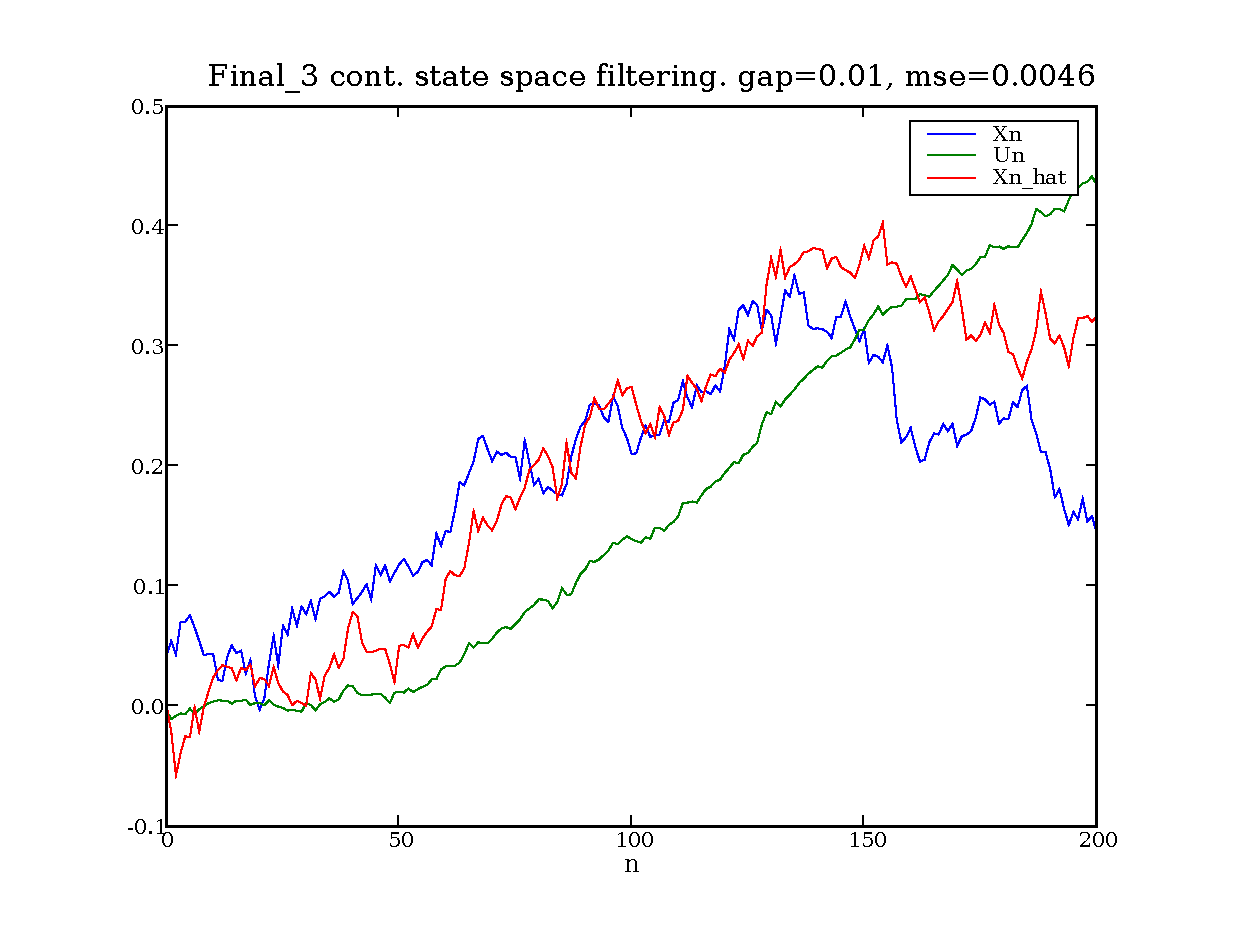
\includegraphics[width=1\textwidth]{Final_3_Xn_Un_Xn_hat_gap_0.01.eps}
\caption{}\label{f1}
\end{figure}

\begin{figure}
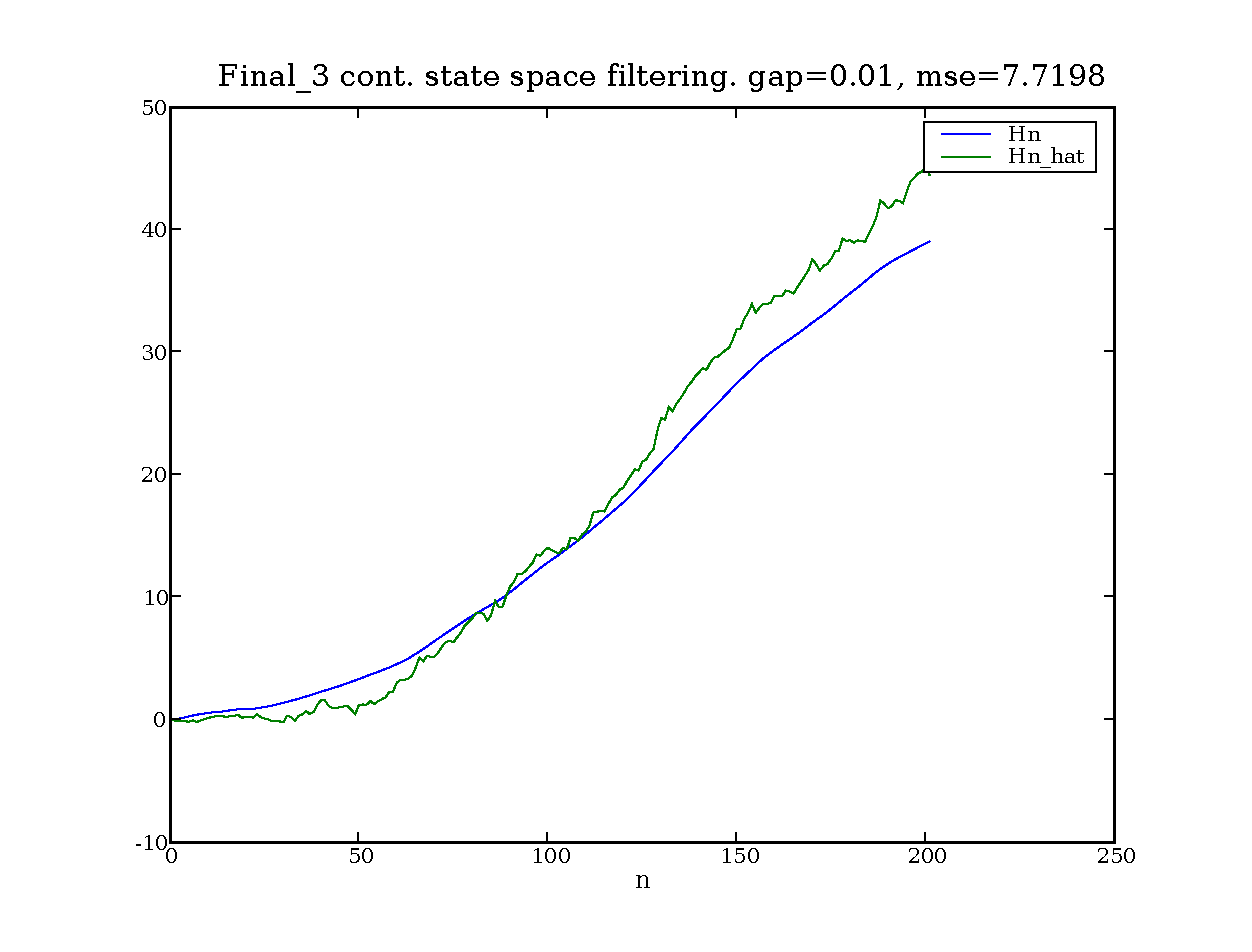
\includegraphics[width=1\textwidth]{Final_3_Hn_Hn_hat_gap_0.01.eps}
\caption{}\label{f2}
\end{figure}

\begin{figure}
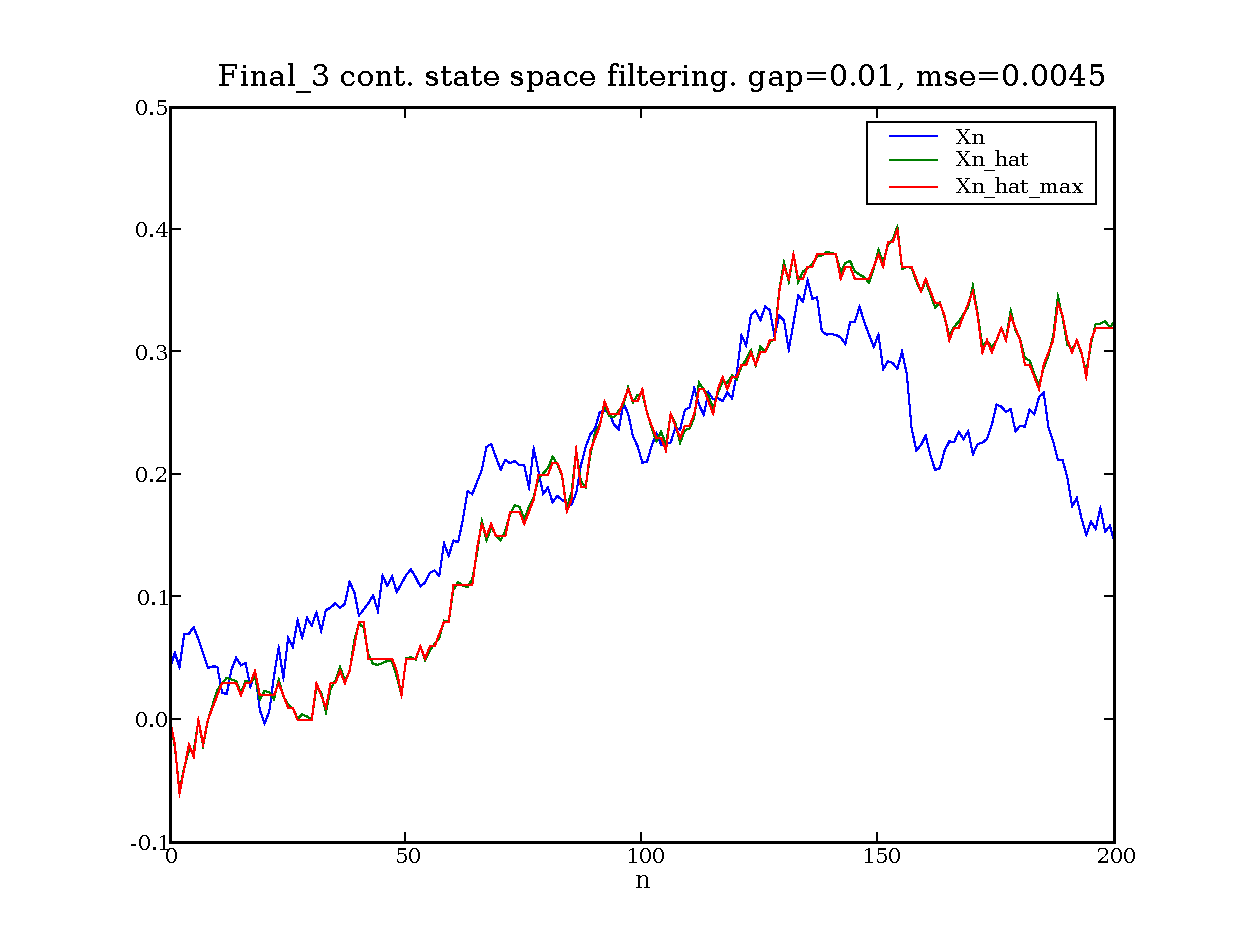
\includegraphics[width=1\textwidth]{Final_3_Xn_Xn_hat_Xn_hat_max_gap_0.01.eps}
\caption{}\label{f3}
\end{figure}

\begin{figure}
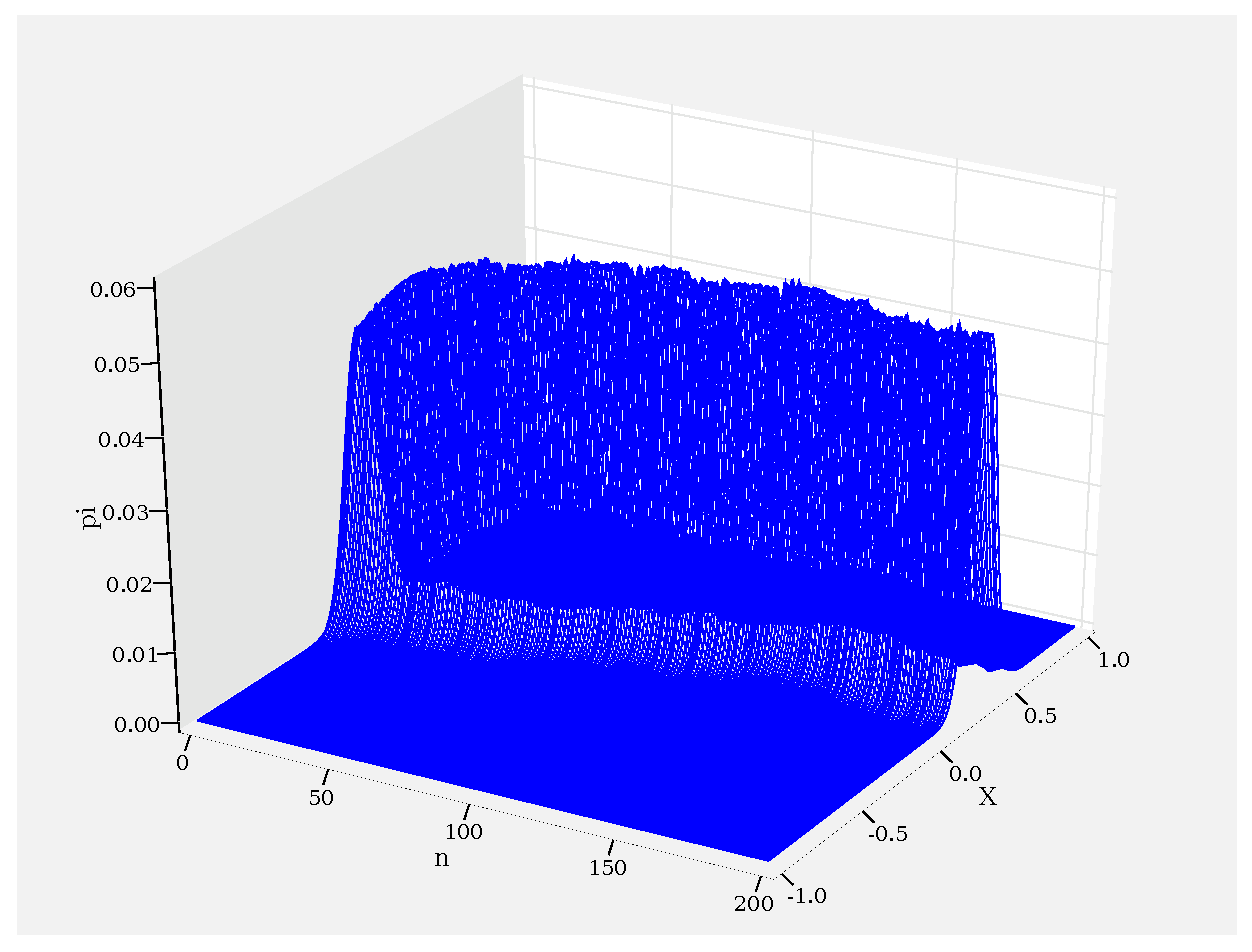
\includegraphics[width=1\textwidth]{Final_3_3d_pi_FDF.eps}
\caption{}\label{f4}
\end{figure}

\begin{figure}
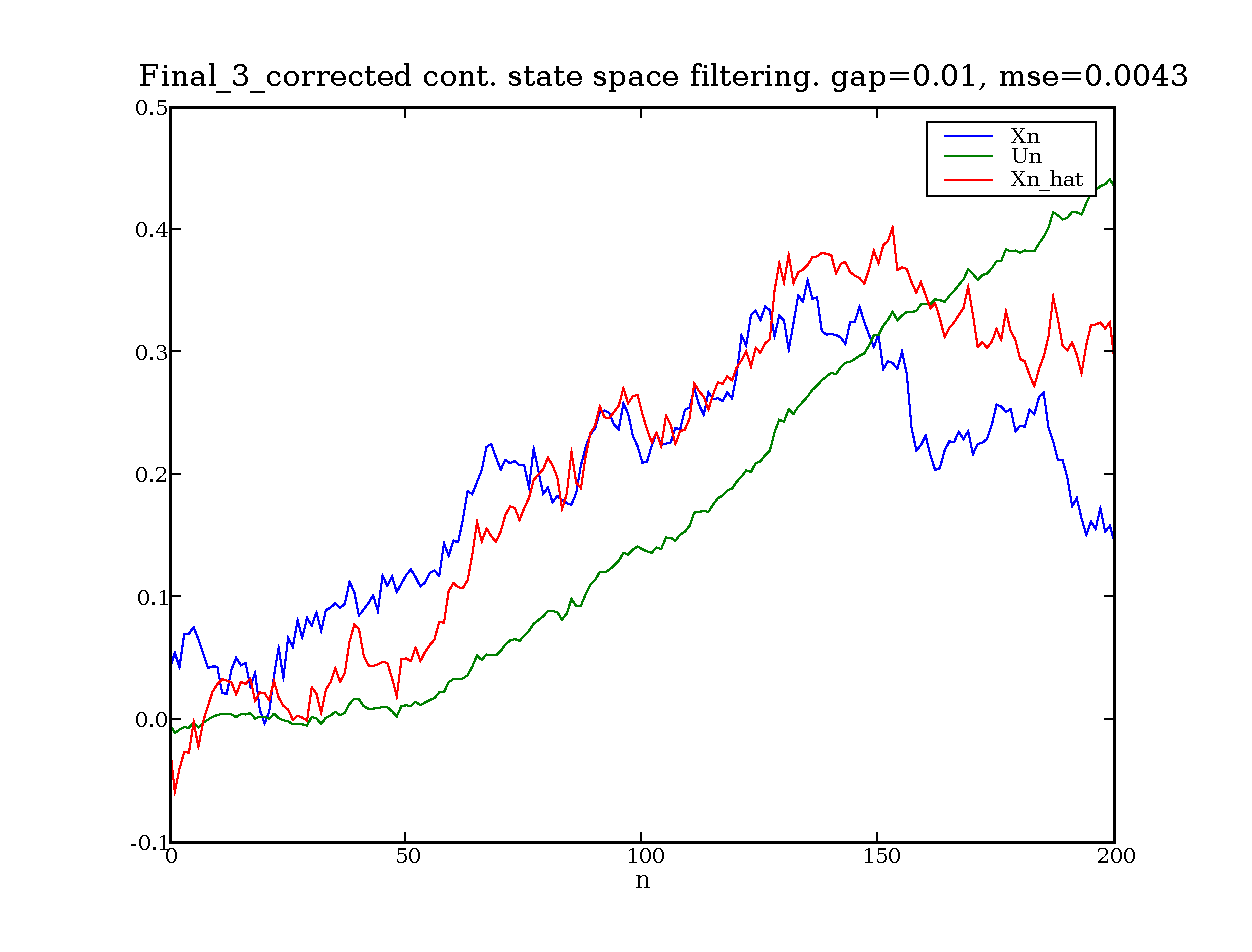
\includegraphics[width=1\textwidth]{Final_3_corrected_Xn_Un_Xn_hat_gap_0.01.eps}
\caption{}\label{f5}
\end{figure}

\begin{figure}
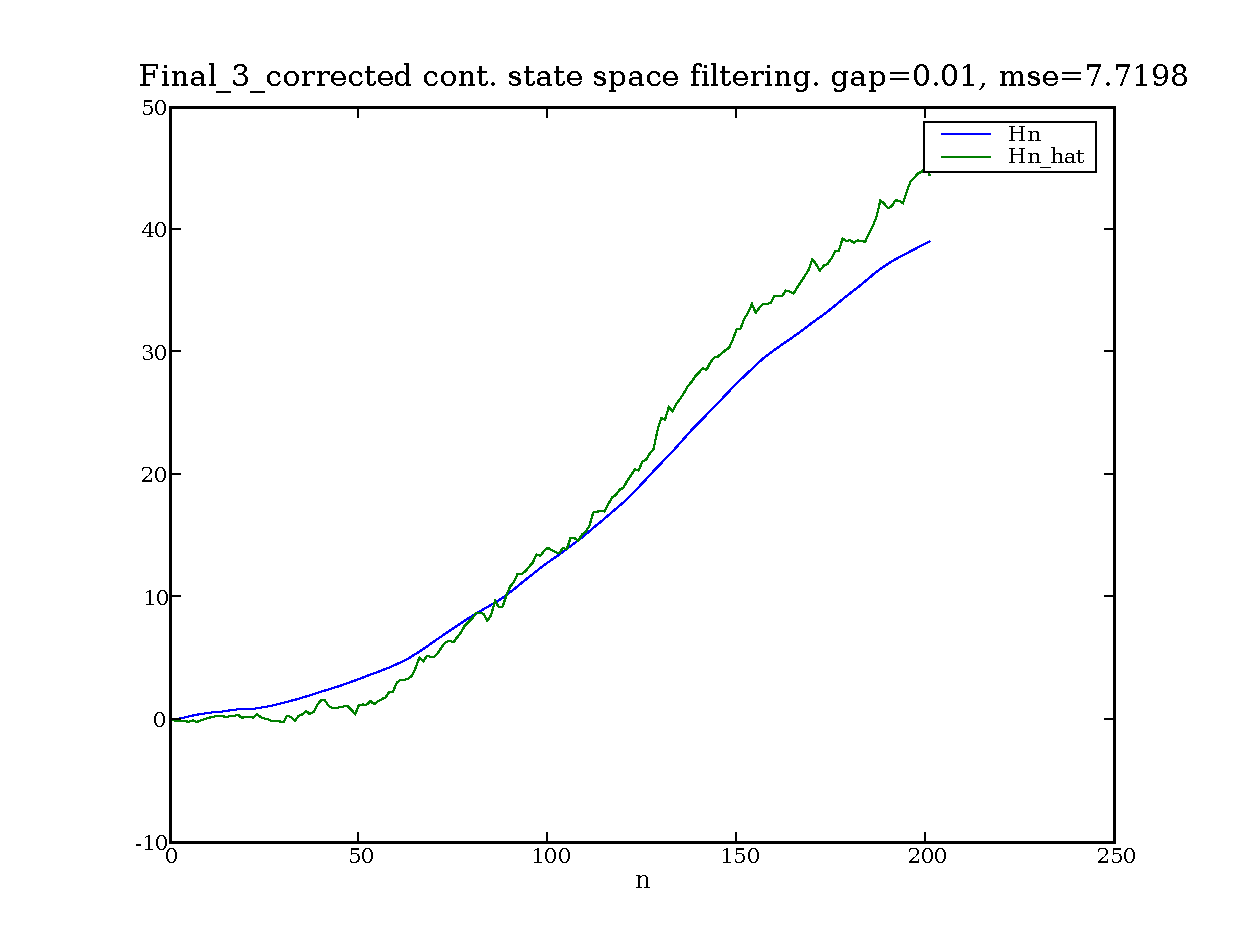
\includegraphics[width=1\textwidth]{Final_3_corrected_Hn_Hn_hat_gap_0.01.eps}
\caption{}\label{f6}
\end{figure}

\begin{figure}
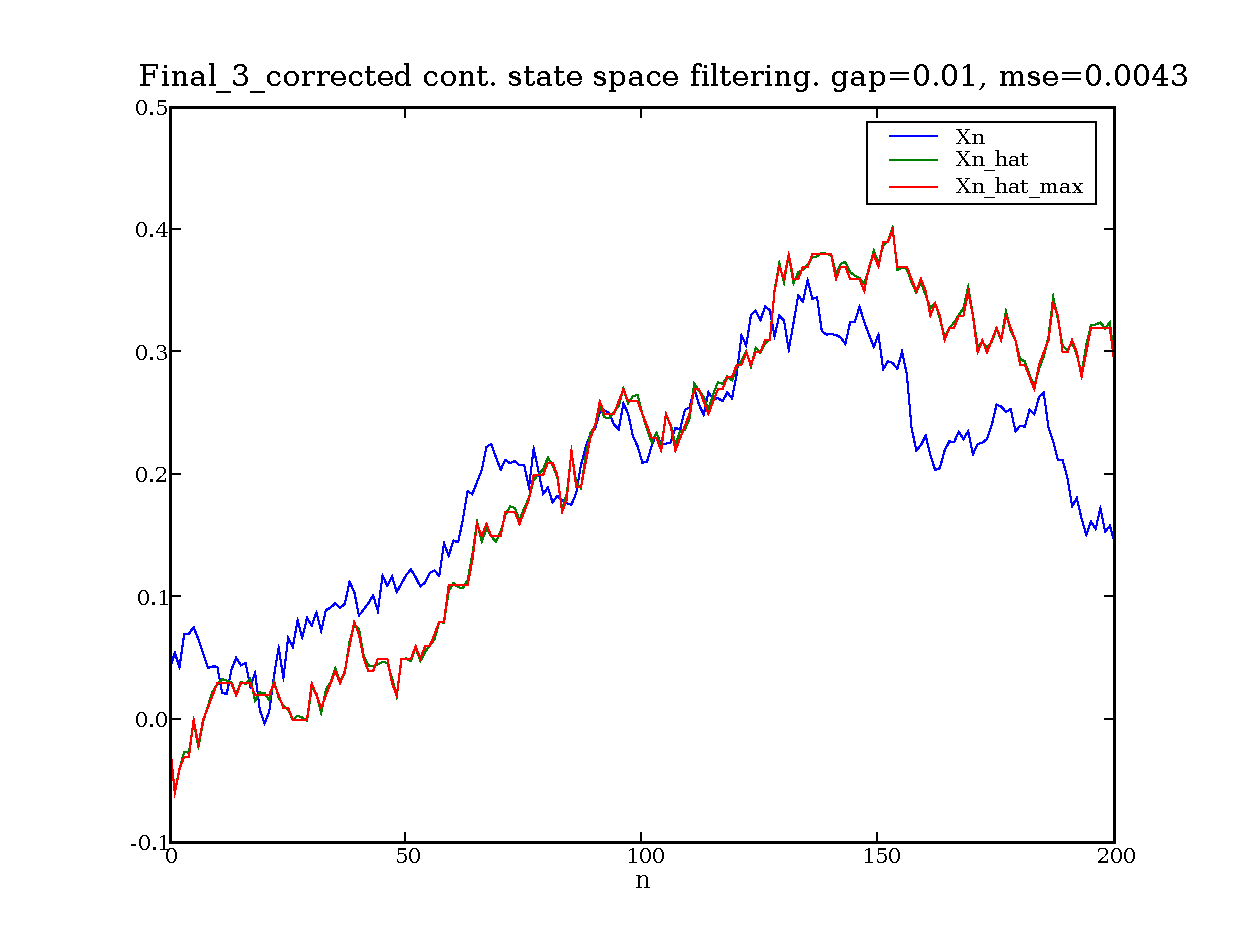
\includegraphics[width=1\textwidth]{Final_3_corrected_Xn_Xn_hat_Xn_hat_max_gap_0.01.eps}
\caption{}\label{f7}
\end{figure}

\begin{figure}
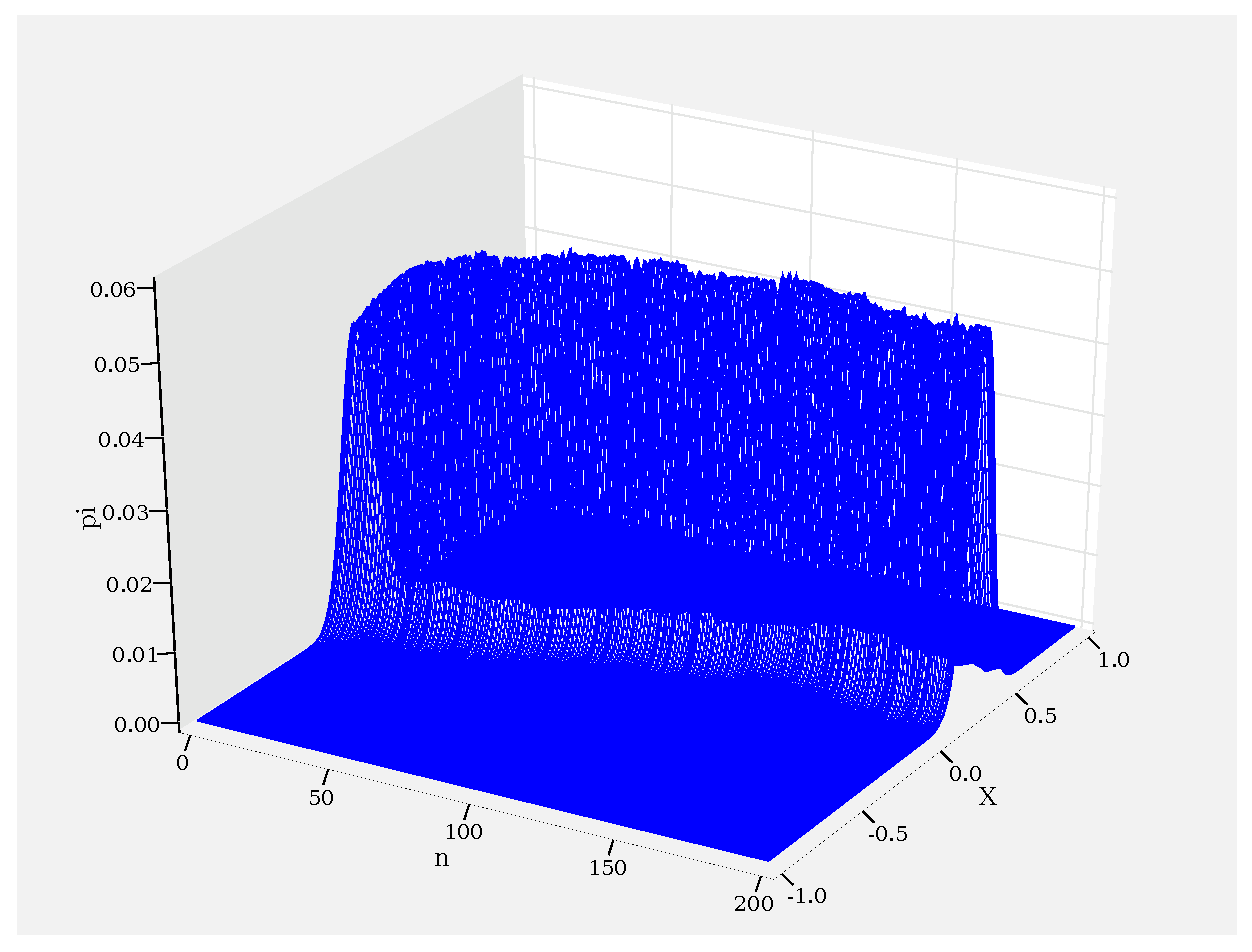
\includegraphics[width=1\textwidth]{Final_3_corrected_3d_pi_FDF.eps}
\caption{}\label{f8}
\end{figure}

\begin{figure}
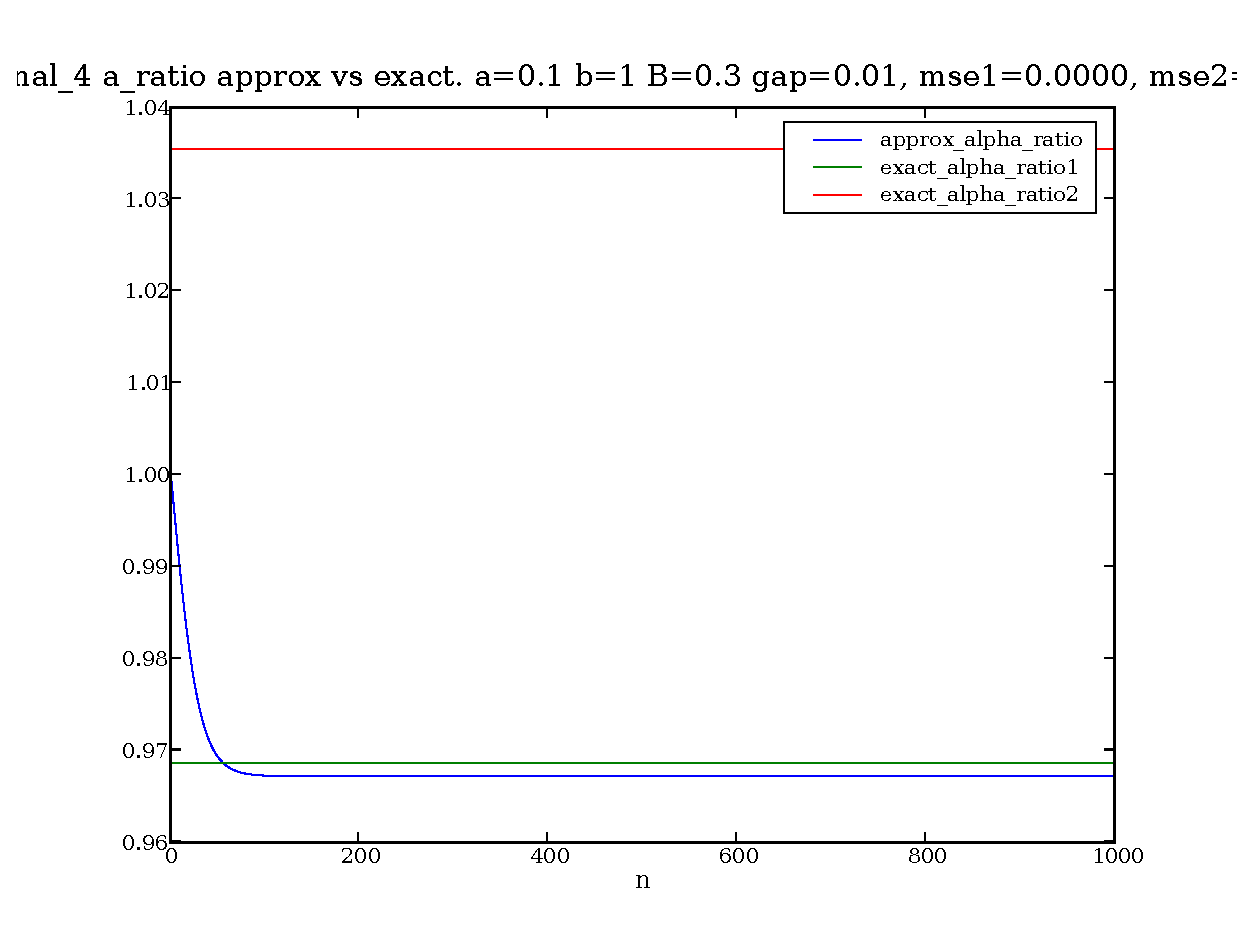
\includegraphics[width=1\textwidth]{Final_4_alpha_ratio_comp_a_0.1_b_1_B_0.3_gap_0.01.eps}
\caption{}\label{f9}
\end{figure}

\begin{figure}
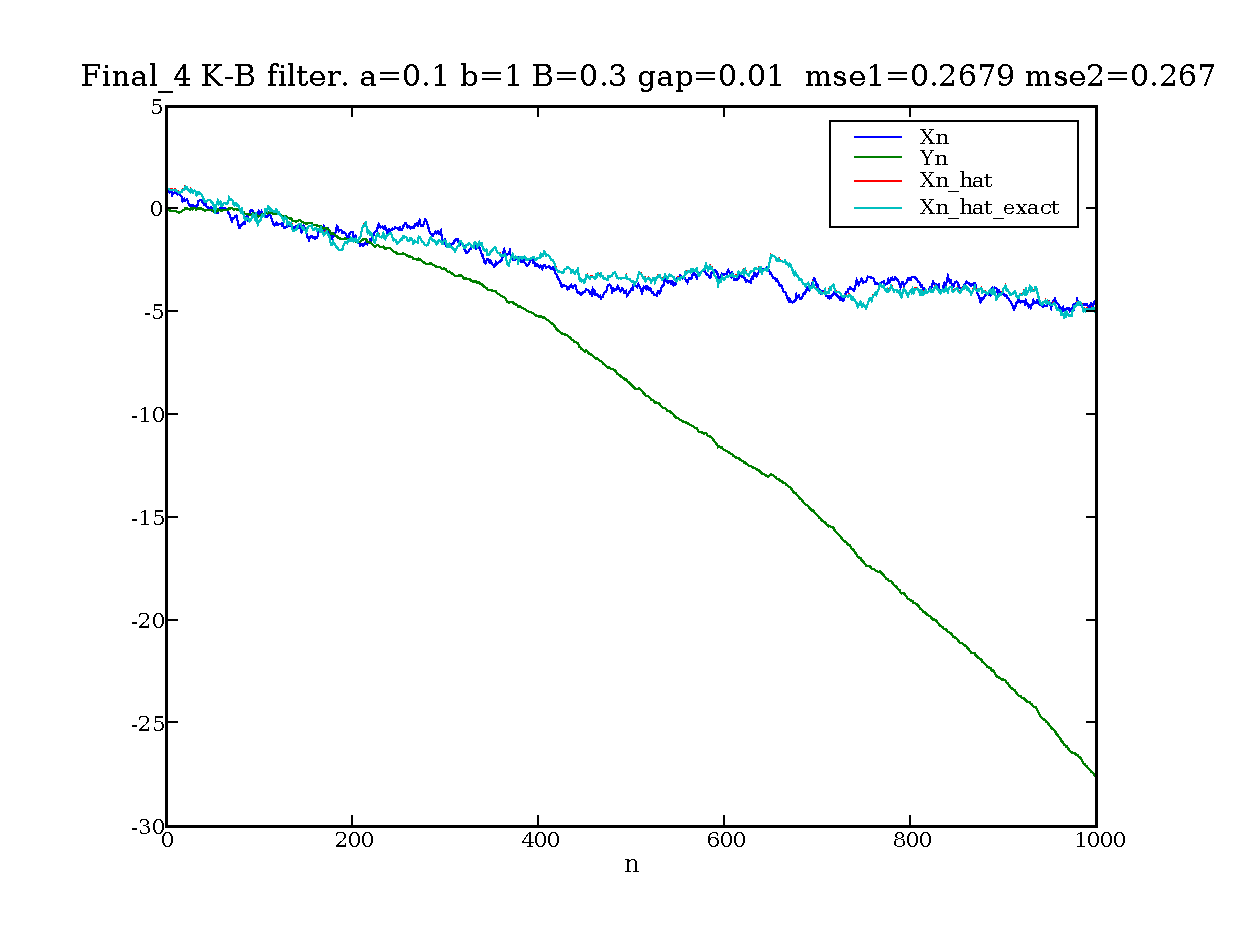
\includegraphics[width=1\textwidth]{Final_4_Xn_Yn_Xn_hat_a_0.1_b_1_B_0.3_gap_0.01.eps}
\caption{}\label{f10}
\end{figure}

\begin{figure}
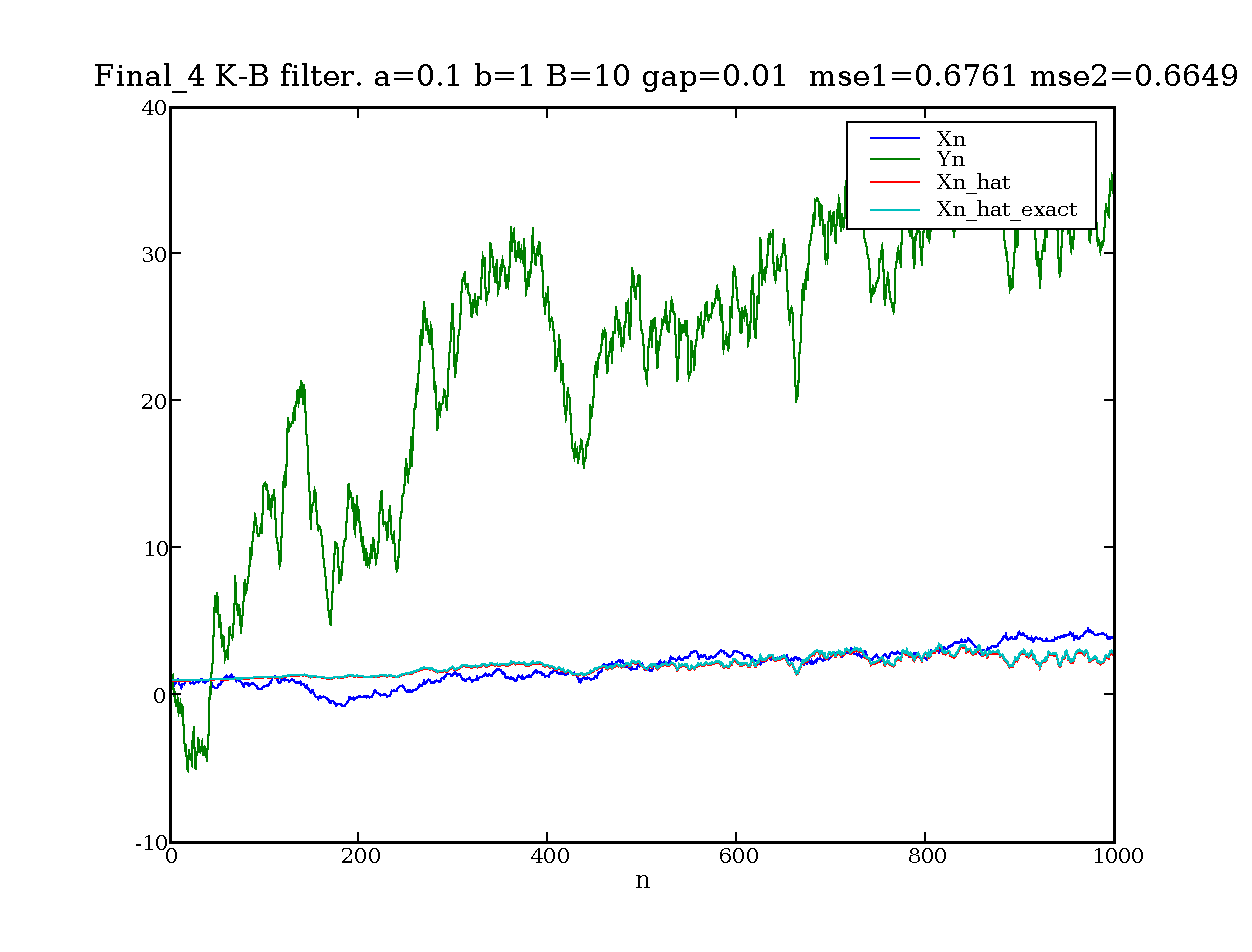
\includegraphics[width=1\textwidth]{Final_4_Xn_Yn_Xn_hat_a_0.1_b_1_B_10_gap_0.01.eps}
\caption{}\label{f11}
\end{figure}

\begin{figure}
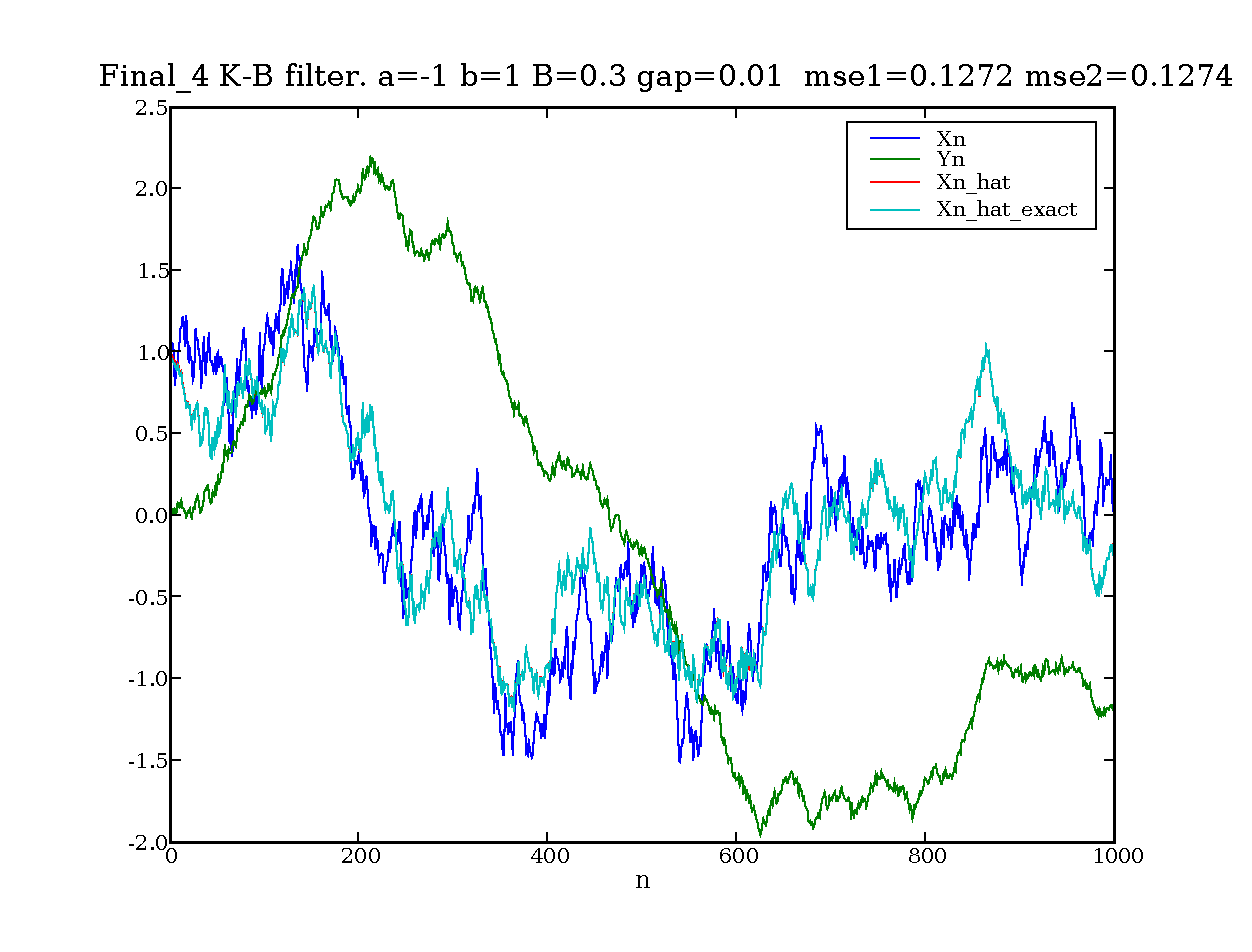
\includegraphics[width=1\textwidth]{Final_4_Xn_Yn_Xn_hat_a_-1_b_1_B_0.3_gap_0.01.eps}
\caption{}\label{f12}
\end{figure}

\begin{figure}
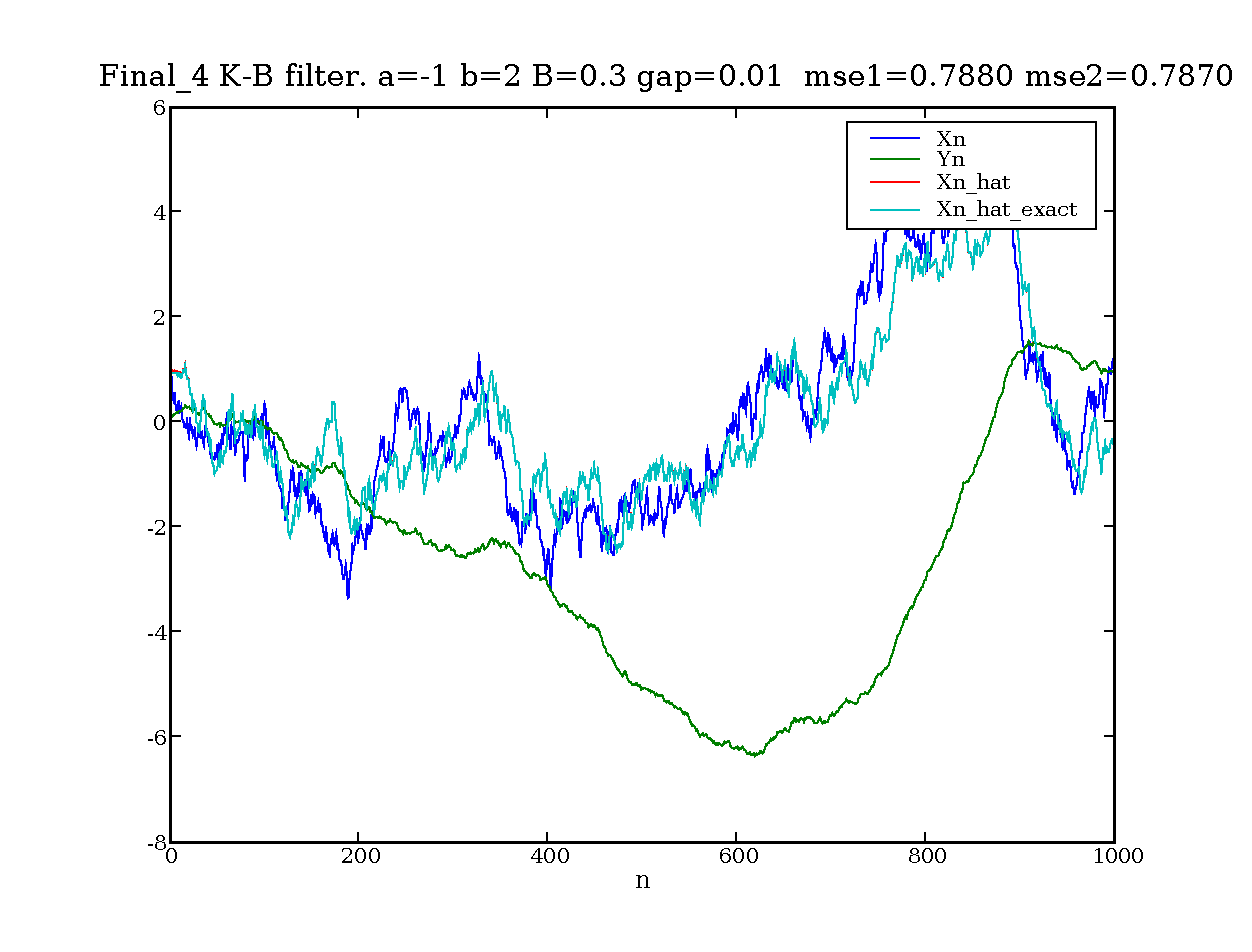
\includegraphics[width=1\textwidth]{Final_4_Xn_Yn_Xn_hat_a_-1_b_2_B_0.3_gap_0.01.eps}
\caption{}\label{f13}
\end{figure}

\end{document}
